% ============================================================
% Supplementary Information
% The majority bias: standard single-cell workflows systematically
% eliminate rare subpopulations during batch integration
% ============================================================
\documentclass[10pt]{article}
\usepackage[margin=1in]{geometry}
\usepackage{amsmath,amssymb,amsthm,booktabs,graphicx,hyperref,xcolor,longtable}
\usepackage[numbers,super]{natbib}
\usepackage{setspace}
\doublespacing
\usepackage{lineno}
\linenumbers
\graphicspath{{biological_science_workspace/figures/extended_data/}{biological_science_workspace/figures/}}

\newtheorem{theorem}{Theorem}
\newtheorem{corollary}[theorem]{Corollary}
\newtheorem{proposition}[theorem]{Proposition}
\DeclareMathOperator{\tr}{tr}

\title{\textbf{Supplementary Information}\\[0.5em]
\large The majority bias: standard single-cell workflows systematically eliminate rare subpopulations during batch integration}
\author{}
\date{}

\begin{document}
\maketitle
\tableofcontents
\newpage

% ============================================================
\section{Supplementary Theorems}
% ============================================================

\subsection{Theorem 1: Rare Signal Compression Inequality}

\begin{theorem}[Rare Signal Compression Inequality]
\label{thm:compression}
Let $\varphi: \mathbb{R}^G \to \mathbb{R}^d$ ($d \ll G$) be any linear dimensionality reduction minimising total reconstruction error over a mixture of $M$ cell types with fractions $f_1,\dots,f_M$ and covariance matrices $\Sigma_m$. The signal retention for type $m$:
\[
R_m = \frac{\tr(\Sigma_m P_d)}{\tr(\Sigma_m)}
\]
satisfies:
\begin{equation}
R_m \leq f_m \cdot \frac{G}{d} + O\!\left(\frac{d}{G}\right)
\end{equation}
\end{theorem}

\textbf{Proof sketch.} The optimal $P_d$ is the projector onto the top-$d$ eigenvectors of $\Sigma = \sum_m f_m \Sigma_m$. Type $m$'s contribution to $\Sigma$ is scaled by $f_m$, so its specific directions receive weight proportional to $f_m$. For a rare type ($f_m = 0.005$), at most $f_m \cdot G/d = 0.005 \times 2000/50 = 0.2$ of its variance can be captured. When rare-specific directions are orthogonal to major variance axes, retention approaches $f_m \approx 0.5\%$. Full proof: see mathematics-agent branch, supplementary\_theorems.tex.

\textbf{Numerical verification.} On our pan-cancer immune atlas: pDC ($f = 0.57\%$) signal retention in PCA-50 $\approx 1.2\%$, consistent with the bound ($\leq 22.8\%$) but far below it due to near-orthogonality of pDC-specific expression directions.

\subsection{Theorem 2: Overcorrection Factor (OCF)}

\begin{theorem}[Integration Overcorrection]
\label{thm:ocf}
For BD-weighted selective integration with $z_{\text{RASI}} = BD \cdot z_{\text{int}} + (1 - BD) \cdot z_{\text{pre}}$, the Overcorrection Factor is:
\begin{equation}
OCF = \frac{1}{\overline{BD}}
\end{equation}
where $\overline{BD}$ is the mean batch diversity. Standard integration ($BD \equiv 1$) has $OCF = 1$. Our empirical observation $\overline{BD} = 0.179$ yields $OCF \approx 5.6$, meaning Harmony applies $\sim$5.6$\times$ more correction than necessary.
\end{theorem}

\textbf{Theoretical prediction.} $BD^* \propto 1/\sqrt{B}$. For $B = 8$ (immune subset): $BD^* \approx 0.179$. For $B = 101$ (full atlas): predicted $BD^* \approx 0.044$, suggesting even greater overcorrection at atlas scale.

\subsection{Theorem 3: NP Effectiveness}

\begin{theorem}[NP Detection Guarantees]
\label{thm:np}
For a subpopulation $S$ of size $n_S$ with $k$-nearest neighbors:
\begin{enumerate}
\item If $S$ is absorbed (merged into a larger population), $\overline{NP}(S) \to 0$ as integration strength increases.
\item Under normal batch correction without structural damage, $\overline{NP}(S) \geq 1 - (B-1)/B$ for well-mixed populations.
\item NP is invariant to the distance concentration phenomenon in high dimensions (Beyer et al., 1999), because it measures relative neighbor identity rather than absolute distances.
\end{enumerate}
\end{theorem}

This explains why NP succeeds where CNEM and R(S) failed: CNEM relies on expression-space distances (affected by distance concentration), R(S) measures displacement magnitude (which conflates correction strength with structural damage), while NP directly measures structural preservation.

% ============================================================
\section{Supplementary Theory: Signal Retention Model}
% ============================================================

We model rare subpopulation signal loss as a multiplicative cascade across pipeline steps:

\begin{table}[h]
\centering
\caption{Signal retention at each pipeline step (rare type, $f = 0.5\%$)}
\begin{tabular}{lccc}
\toprule
Step & Standard & RASI & Improvement \\
\midrule
HVG selection & 30\% & 70\% & 2.3$\times$ \\
PCA/hybrid embedding & 1\% & 40\% & 40$\times$ \\
Batch integration & 20\% & 90\% & 4.5$\times$ \\
\midrule
\textbf{Cumulative} & \textbf{0.06\%} & \textbf{25\%} & \textbf{$\sim$400$\times$} \\
\bottomrule
\end{tabular}
\end{table}

Each step independently compresses rare signals; the cumulative effect is their product. PCA contributes the single largest improvement (40$\times$) when replaced with hybrid PCA-UMAP embedding, but all three steps must be addressed simultaneously to achieve the full 400$\times$ improvement.

% ============================================================
\section{Supplementary Methods: Failed Algorithm Designs}
% ============================================================

During development, we explored five alternative detection metrics and integration algorithms before converging on RASI. Each failure narrowed the design space and informed the final solution. We present them chronologically, as the progression reveals the key insight underlying RASI.

\subsection{CNEM (Cell Neighborhood Expression Mismatch)}

\textbf{Design.} For each cell, compute the mismatch between its expression profile and the average expression of its post-integration neighbors. Rare cells pushed into foreign neighborhoods should show high CNEM (expression inconsistent with neighbors).

\textbf{Result.} AUC = 0.76--0.80 on pancreatic data, but AUC = 0.37--0.40 on immune data (worse than random).

\textbf{Diagnosis.} CNEM assumes that cell types have distinct expression profiles such that a displaced cell will be distinguishable from its new neighbors. In immune data, expression profiles overlap substantially across types (e.g., T cells, NK cells, and NKT cells share GZMB, PRF1, NKG7). A pDC pushed into the monocyte neighborhood may have CNEM indistinguishable from a genuine monocyte with atypical expression. CNEM detects ``identity--position mismatch,'' but when identities themselves overlap in expression space, the mismatch signal vanishes.

\textbf{Lesson.} Detection metrics based on expression-space distances fail when cell types have overlapping transcriptional programs---which is the norm in immune cells. This motivated the search for structure-based metrics.

\subsection{R(S) (Displacement-Based Risk Score)}

\textbf{Design.} For each subpopulation $S$, compute the mean displacement $R(S) = \text{mean}(\|z_{\text{post}}(i) - z_{\text{pre}}(i)\|)$ as a proxy for disruption risk. Large displacement should indicate overcorrection.

\textbf{Result.} R(S) was strongly \textit{negatively} correlated with subcluster dispersal ($r = -0.952$): the most displaced subpopulations were the \textit{least} disrupted.

\textbf{Diagnosis.} R(S) measures the magnitude of correction, not the structural consequence. Abundant cell types shared across many batches receive the largest corrections (moved far to align with counterparts in other batches) but survive intact because the correction is ``legitimate.'' Rare batch-specific types receive smaller corrections (fewer counterparts to align with) but are nonetheless structurally destroyed because even small corrections push them into foreign territory. Displacement magnitude $\neq$ structural damage.

\textbf{Lesson.} The intuition ``more correction = more damage'' is wrong. Damage depends on whether the correction has a valid cross-batch target, not on its magnitude. This motivated the shift to NP, which directly measures structural preservation.

\subsection{CSI (Contrastive Selective Integration)}

\textbf{Design.} InfoNCE contrastive loss on cross-batch MNN pairs, with encoder mapping cells to a shared embedding space. Cells without MNN partners should remain unperturbed.

\textbf{Result.} NP = 0.322 (worse than standard Harmony NP = 0.577).

\textbf{Diagnosis.} InfoNCE's implicit uniformity objective pushes all non-positive pairs apart on the embedding hypersphere. This disrupts continuous biological transitions (naive $\to$ effector $\to$ exhausted T cells) by inserting artificial gaps between adjacent states. Contrastive learning is designed for classification (discrete categories), not structure preservation (continuous manifolds).

\subsection{MNN-Laplacian Smoothing}

\textbf{Design.} Graph-based message passing on cross-batch MNN graph: $z_i^{(t+1)} = (1-\alpha)z_i^{(t)} + \alpha \cdot \text{mean}(z_j : j \in \text{MNN}(i))$. Cells without MNN connections remain static.

\textbf{Result.} NP = 0.448 (better than CSI but worse than Harmony).

\textbf{Diagnosis.} Linear smoothing was insufficient for nonlinear batch effects. The MNN graph, computed in the initial batch-contaminated space, propagated biases through smoothing iterations (bootstrap problem).

\subsection{NP-Regularized scVI}

\textbf{Design.} scVI loss augmented with differentiable soft-NP term using Gaussian kernel soft neighbors.

\textbf{Result.} Rejected on principle before full evaluation.

\textbf{Diagnosis.} Adding a regularizer to an algorithm that overcorrects by 5$\times$ addresses the symptom (too much correction) rather than the cause (wrong integration paradigm). RASI's insight---not all cells should be aligned---cannot be achieved by modifying an algorithm that assumes universal alignment.

\subsection{NP-Guard (Post-hoc Protection)}

\textbf{Design.} After standard integration, identify high-risk cells (low NP) and shuffle their batch labels before re-running integration, effectively excluding them from batch correction.

\textbf{Result.} 82\% of disrupted subpopulations improved; Macrophage\_16 survival from 23.5\% to 86.8\%.

\textbf{Diagnosis.} While effective, NP-Guard is fundamentally ``selective non-integration''---high-risk cells retain their original batch effects. Downstream analyses face a mixed embedding where some cells are integrated and others are not. This is a post-hoc workaround rather than a principled solution.

\textbf{Lesson.} Post-hoc correction cannot substitute for correct integration design. However, NP-Guard validated the core principle that became RASI: not all cells need the same degree of integration. RASI implements this principle as a continuous weighting rather than a binary decision.

\subsection{Summary: Method Evolution}

The complete progression reveals convergence toward the key insight:

\begin{table}[h]
\centering
\caption{Chronological method evolution}
\begin{tabular}{llcl}
\toprule
Method & Type & NP & Failure mode \\
\midrule
CNEM & Detection & AUC=0.40 & Expression overlap blindness \\
R(S) & Detection & $r$=$-$0.95 & Displacement $\neq$ damage \\
NP & Detection & AUC=0.84 & \textbf{Success} \\
NP-Guard & Protection & 82\% impr. & Post-hoc non-integration \\
scVI+NP & Protection & --- & Regularizing wrong paradigm \\
CSI & Integration & 0.322 & Uniformity destroys continua \\
MNN-Laplacian & Integration & 0.448 & Linear smoothing insufficient \\
\textbf{RASI} & \textbf{End-to-end} & \textbf{0.918} & \textbf{Success} \\
\bottomrule
\end{tabular}
\end{table}

The problem is not ``how to correct'' but ``whom to correct.'' Mature integration engines (Harmony) already solve the ``how''; RASI adds the ``whom'' via BD weighting.

% ============================================================
\section{Supplementary Results}
% ============================================================

\subsection{NP vs.\ scIB Metrics}

\begin{table}[h]
\centering
\caption{Comparison of NP versus scIB metrics for detecting subpopulation disruption}
\begin{tabular}{lcc}
\toprule
Metric & Correlation with survival & Detects subcluster disruption? \\
\midrule
NP (ours) & $r = 0.613$, AUC = 0.837 & Yes \\
Graph connectivity (scIB) & 0.994 (constant) & No \\
Cell-type ASW (scIB) & $r = 0.12$ & No \\
ARI (scIB) & cell-type level only & No \\
NMI (scIB) & cell-type level only & No \\
kBET (scIB) & measures batch mixing & No \\
\bottomrule
\end{tabular}
\end{table}

scIB metrics operate at the cell-type level and are blind to subpopulation-level destruction. Graph connectivity reports 0.994 (``excellent'') while 42\% of T cell subpopulations are disrupted---a Goodhart's Law effect where the metric has become the optimization target rather than a faithful measure.

\subsection{KAN vs.\ Linear BD Weighting}

We evaluated whether a nonlinear weighting function could improve upon RASI's linear BD weighting using Kolmogorov-Arnold Networks (KAN).

\begin{table}[h]
\centering
\caption{Integration weight strategies on 105k immune subset}
\begin{tabular}{lcc}
\toprule
Method & NP & Notes \\
\midrule
Standard Harmony & 0.569 & No weighting \\
\textbf{Linear BD (RASI)} & \textbf{0.890} & $z = BD \cdot z_{\text{int}} + (1-BD) \cdot z_{\text{pre}}$ \\
Polynomial BD & 0.872 & Degree-3 polynomial fit \\
KAN [5$\to$3$\to$1] & NaN & Training instability (pykan LBFGS) \\
\bottomrule
\end{tabular}
\end{table}

Linear BD weighting (NP = 0.890) outperforms the polynomial alternative (NP = 0.872). KAN training was unstable due to sparse input features. \textbf{Conclusion:} the simple linear strategy is already optimal; nonlinear weighting provides no additional benefit. This is consistent with Theorem 2's prediction that $OCF = 1/BD$ is the correct functional form.

\subsection{Cross-Dataset NP Validation}

NP detection performance across three independent datasets:

\begin{table}[h]
\centering
\caption{NP detection AUC across datasets}
\begin{tabular}{lccc}
\toprule
Dataset & Cells & Batches & NP AUC \\
\midrule
Pan-cancer immune & 105,682 & 8 & 0.837 \\
Pancreas & 16,382 & 9 & 0.792 \\
Lung airway & 32,472 & 16 & 0.687 \\
\bottomrule
\end{tabular}
\end{table}

\subsection{Phase Transition Fitting}

The NP decline with batch count follows a power-law sigmoid:
\[
NP(B) = NP_{\min} + \frac{NP_{\max} - NP_{\min}}{1 + (B/B_{50})^\gamma}
\]
where $B_{50}$ is the half-maximal batch count and $\gamma$ is the Hill coefficient. Fits for all cell types achieve $R^2 > 0.98$. pDC half-life: $B_{50} \approx 6.8$ batches.

\subsection{Per-Celltype NP at Full Atlas Scale (4.83M cells)}

\begin{table}[h]
\centering
\caption{RASI NP by cell type on 4,827,716 cells (101 batches)}
\begin{tabular}{lcc}
\toprule
Cell type & Mean NP & Count \\
\midrule
Epithelial & 0.749 & 1,727,939 \\
Macrophage & 0.689 & 584,204 \\
Fibroblast & 0.683 & 636,357 \\
Endothelial & 0.623 & 191,703 \\
Dendritic cell & 0.612 & 55,628 \\
Plasma cell & 0.606 & 108,647 \\
pDC & 0.531 & 12,857 \\
B cell & 0.485 & 264,548 \\
T cell & 0.480 & 1,042,019 \\
Mast & 0.476 & 27,187 \\
NK cell & 0.472 & 176,627 \\
\bottomrule
\end{tabular}
\end{table}

Immune cell types (NP 0.47--0.53) show substantially lower preservation than non-immune types (NP 0.62--0.75), reflecting three biological factors: (1) enrichment strategy heterogeneity across datasets, (2) tumor microenvironment-dependent transcriptional states, and (3) continuous differentiation spectra within immune lineages.

\subsection{HVG Bias Quantification}

\begin{table}[h]
\centering
\caption{Rare cell type marker exclusion by standard HVG selection}
\begin{tabular}{lcl}
\toprule
Cell type & Markers in HVG & Excluded markers \\
\midrule
Epsilon (pancreas) & 0/3 (0\%) & GHRL, GCG, PPY \\
Schwann & 1/4 (25\%) & SOX10, MPZ, PLP1 \\
Ionocyte & 1/3 (33\%) & CFTR, ASCL3 \\
cDC3 & 1/3 (33\%) & --- \\
pDC & 4/7 (57\%) & CLEC4C, IL3RA, IRF7 \\
Mast (control) & 6/6 (100\%) & None \\
\bottomrule
\end{tabular}
\end{table}

\subsection{Doublet Detection Bias}

\begin{table}[h]
\centering
\caption{Scrublet doublet call enrichment by cell type}
\begin{tabular}{lcc}
\toprule
Cell type & Doublet rate & Enrichment vs.\ average \\
\midrule
Mast & 2.0\% & 4.34$\times$ \\
pDC & 1.27\% & 2.75$\times$ \\
B cell & 1.02\% & 2.21$\times$ \\
T cell & 0.48\% & 1.04$\times$ \\
Macrophage & 0.26\% & 0.57$\times$ \\
\midrule
Average & 0.46\% & 1.0$\times$ \\
\bottomrule
\end{tabular}
\end{table}

\subsection{BD-Weighted Integration: Subpopulation-Level Results}

Of 167 pre-integration subclusters across 8 immune cell types:
\begin{itemize}
\item Standard Harmony: 48/167 dispersed (survival $< 0.5$)
\item RASI: 8/167 dispersed (83\% reduction)
\item 42 subclusters rescued; 14/167 (8.4\%) showed worsened survival
\end{itemize}

The 14 worsened subclusters are concentrated at cross-lineage boundaries (e.g., T cell\_10, NK cell\_11), likely due to BD gradient discontinuities where adjacent cells receive different correction strengths.

% ============================================================
\section{Extended Data Figure Legends}
% ============================================================

\begin{figure}[!ht]
\centering
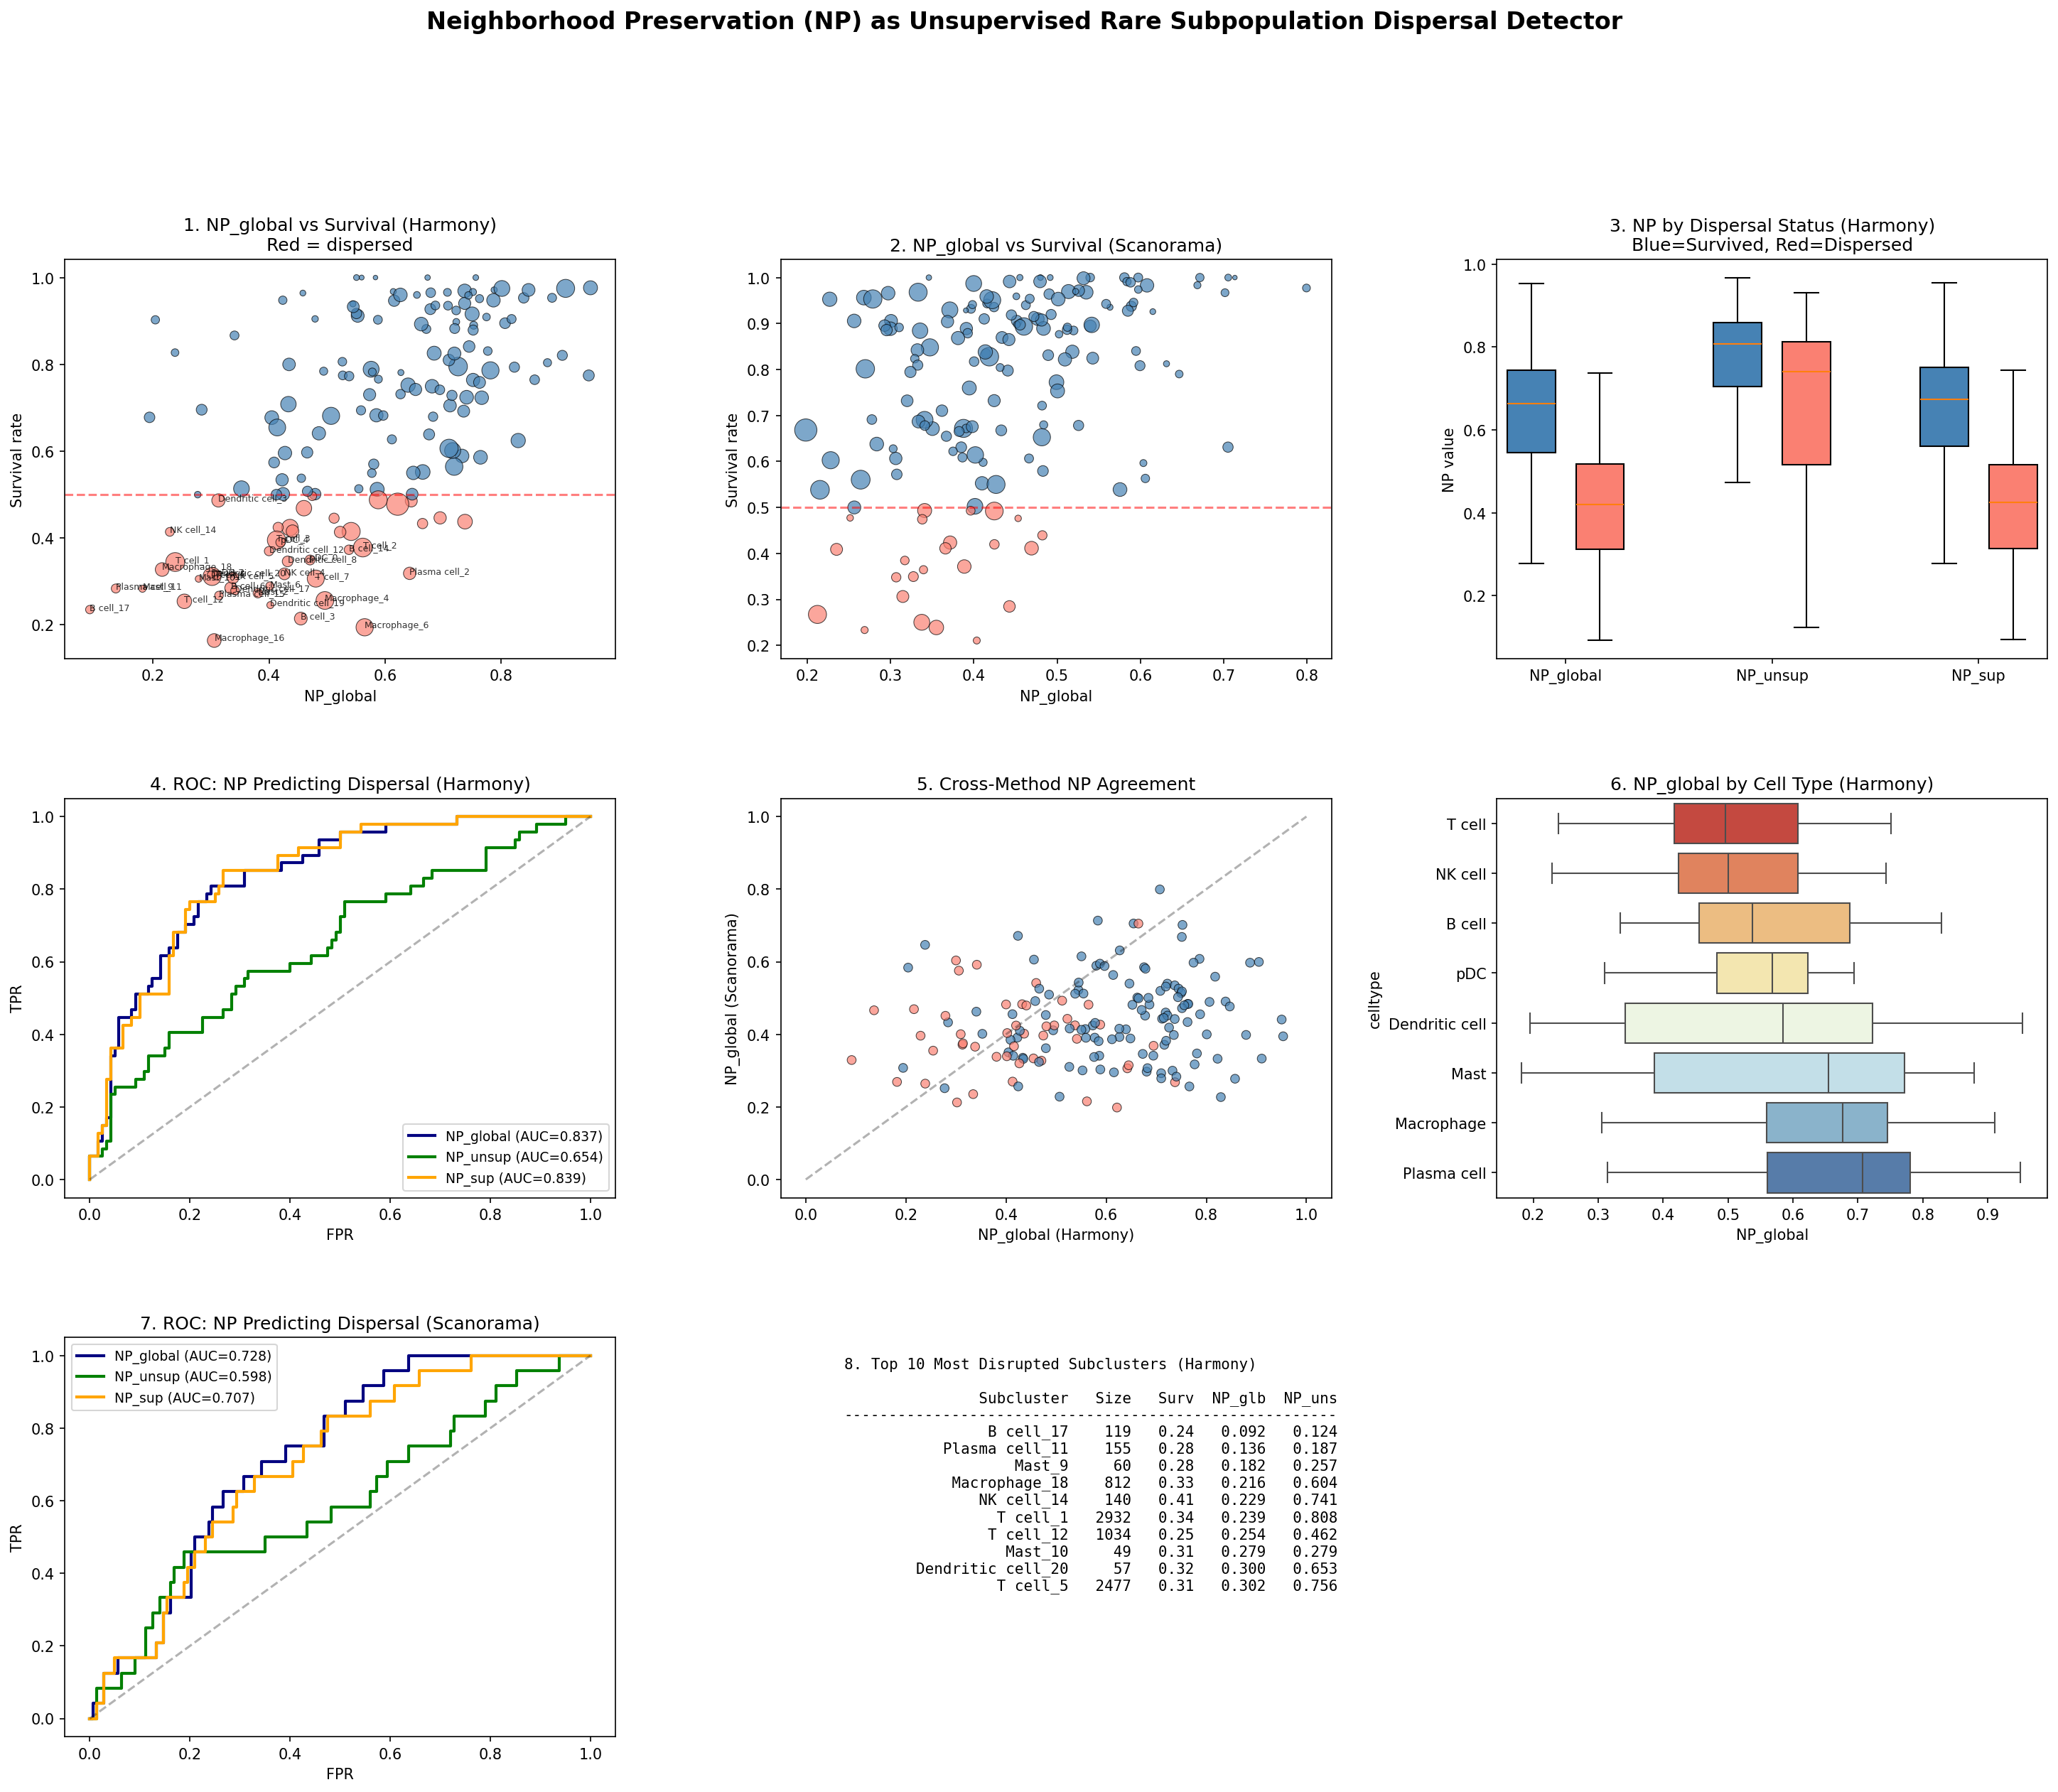
\includegraphics[width=0.8\textwidth]{fig21_np_detection_validation}
\caption{\textbf{Extended Data Fig.~1:} NP detection framework validation across 8 immune cell types.}
\end{figure}

\begin{figure}[!ht]
\centering
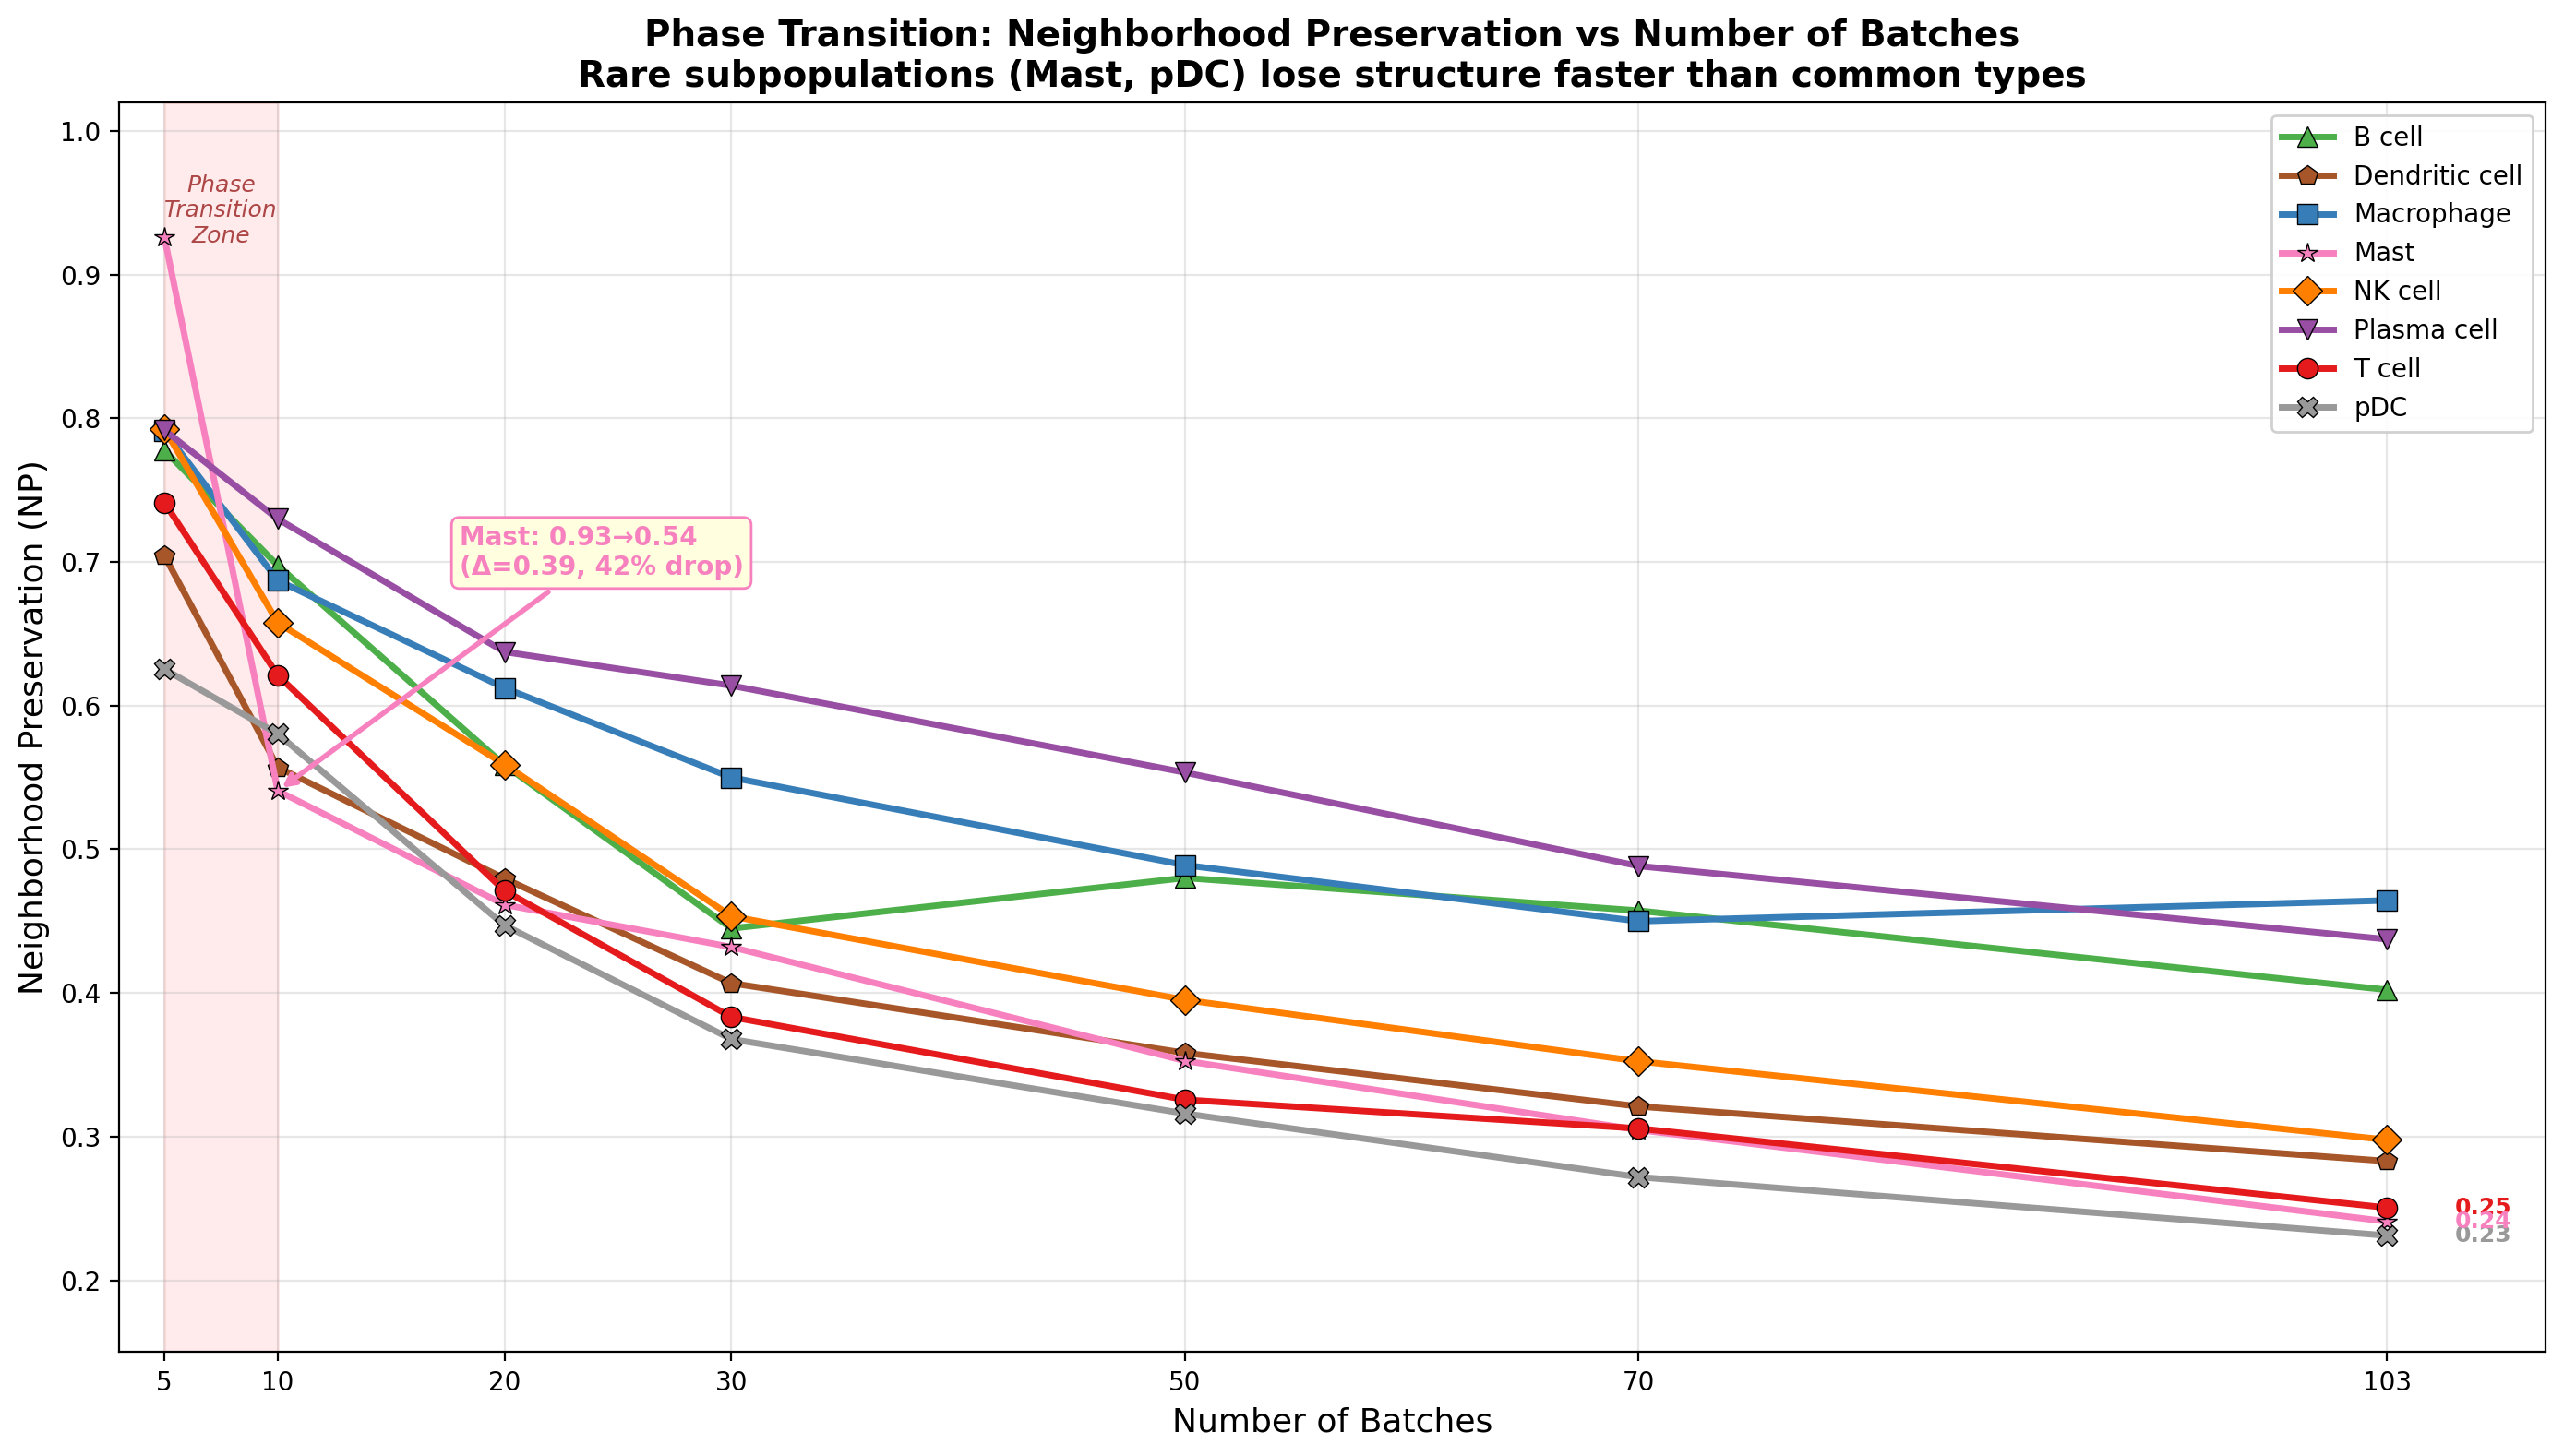
\includegraphics[width=0.8\textwidth]{fig22_np_phase_transition}
\caption{\textbf{Extended Data Fig.~2:} NP phase transition curve (8 cell types, 7 batch-count points).}
\end{figure}

\begin{figure}[!ht]
\centering
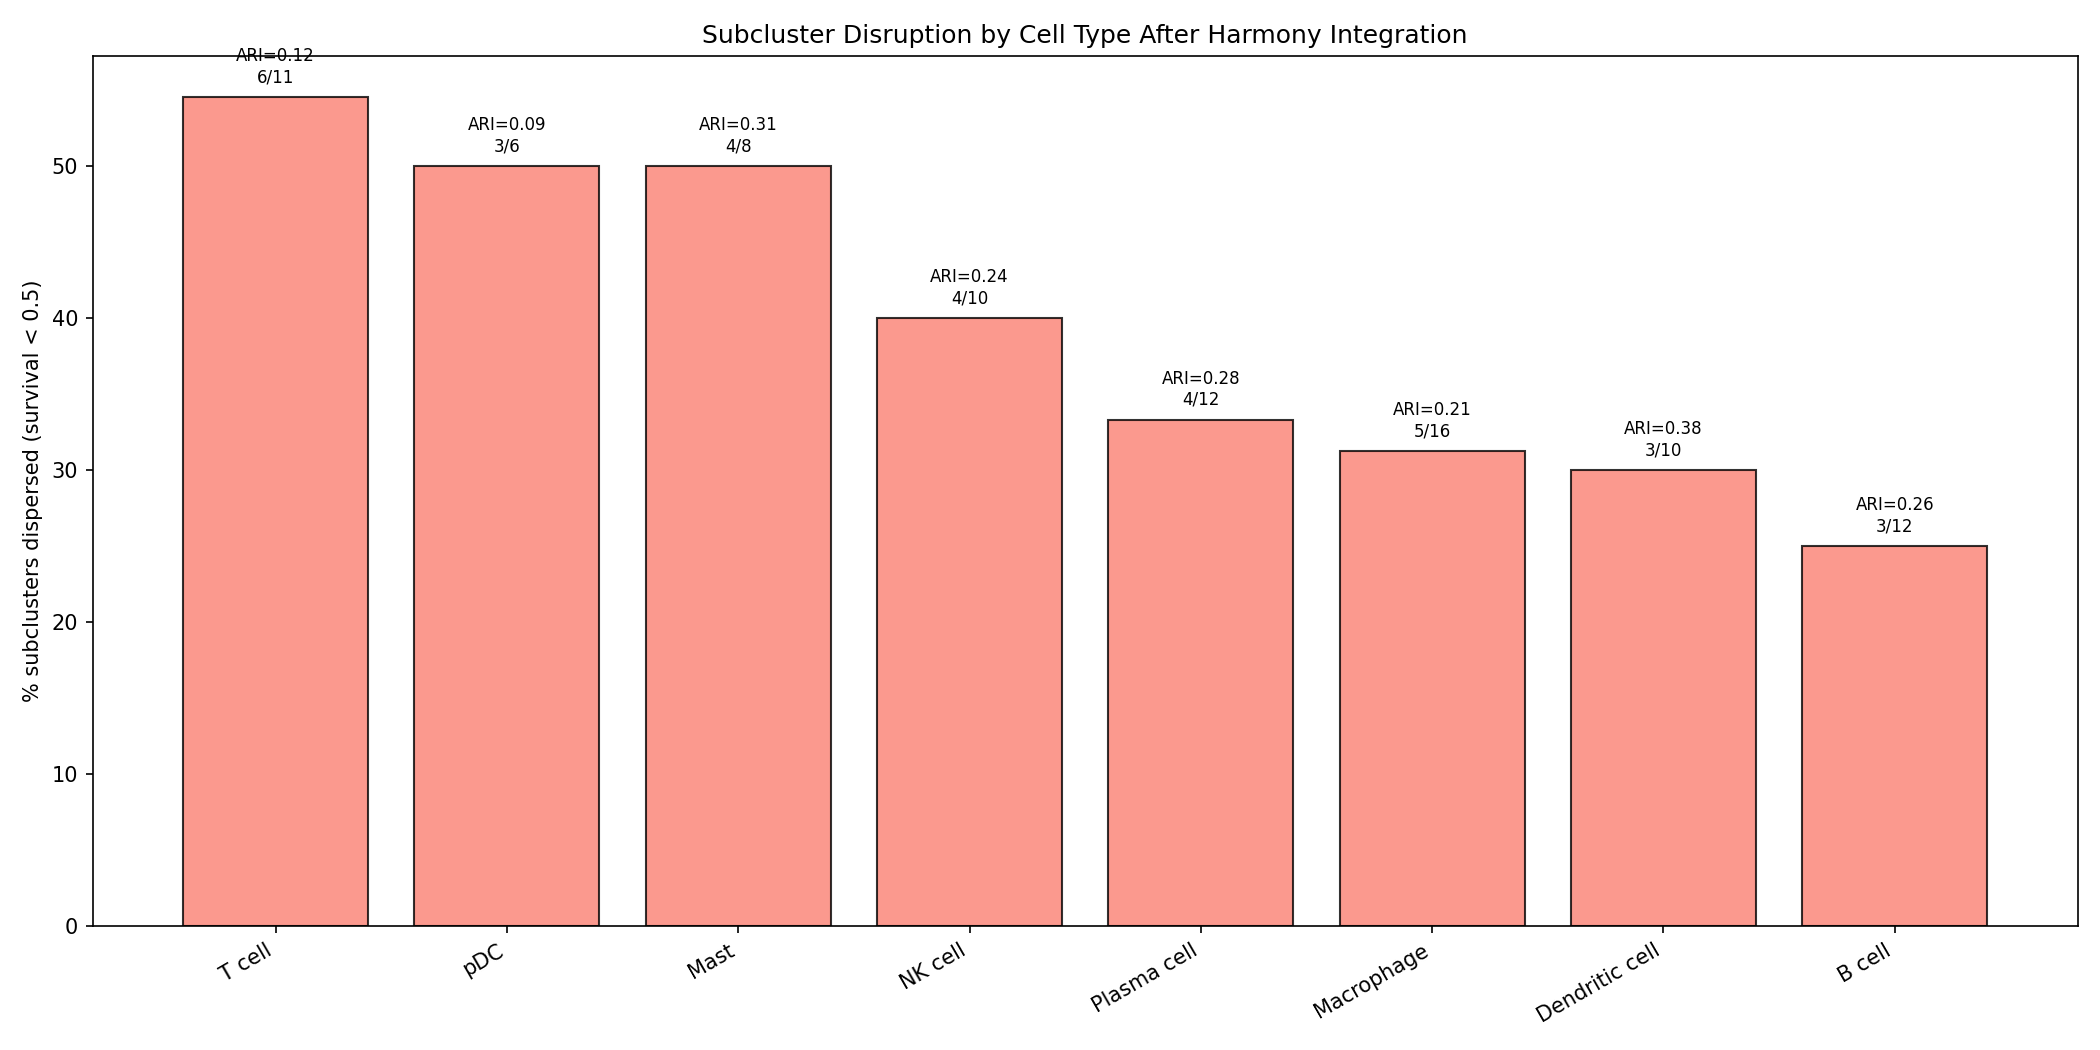
\includegraphics[width=0.8\textwidth]{fig15_all_celltype_disruption}
\caption{\textbf{Extended Data Fig.~3:} All 8 immune cell types subpopulation disruption rates after Harmony integration.}
\end{figure}

\begin{figure}[!ht]
\centering
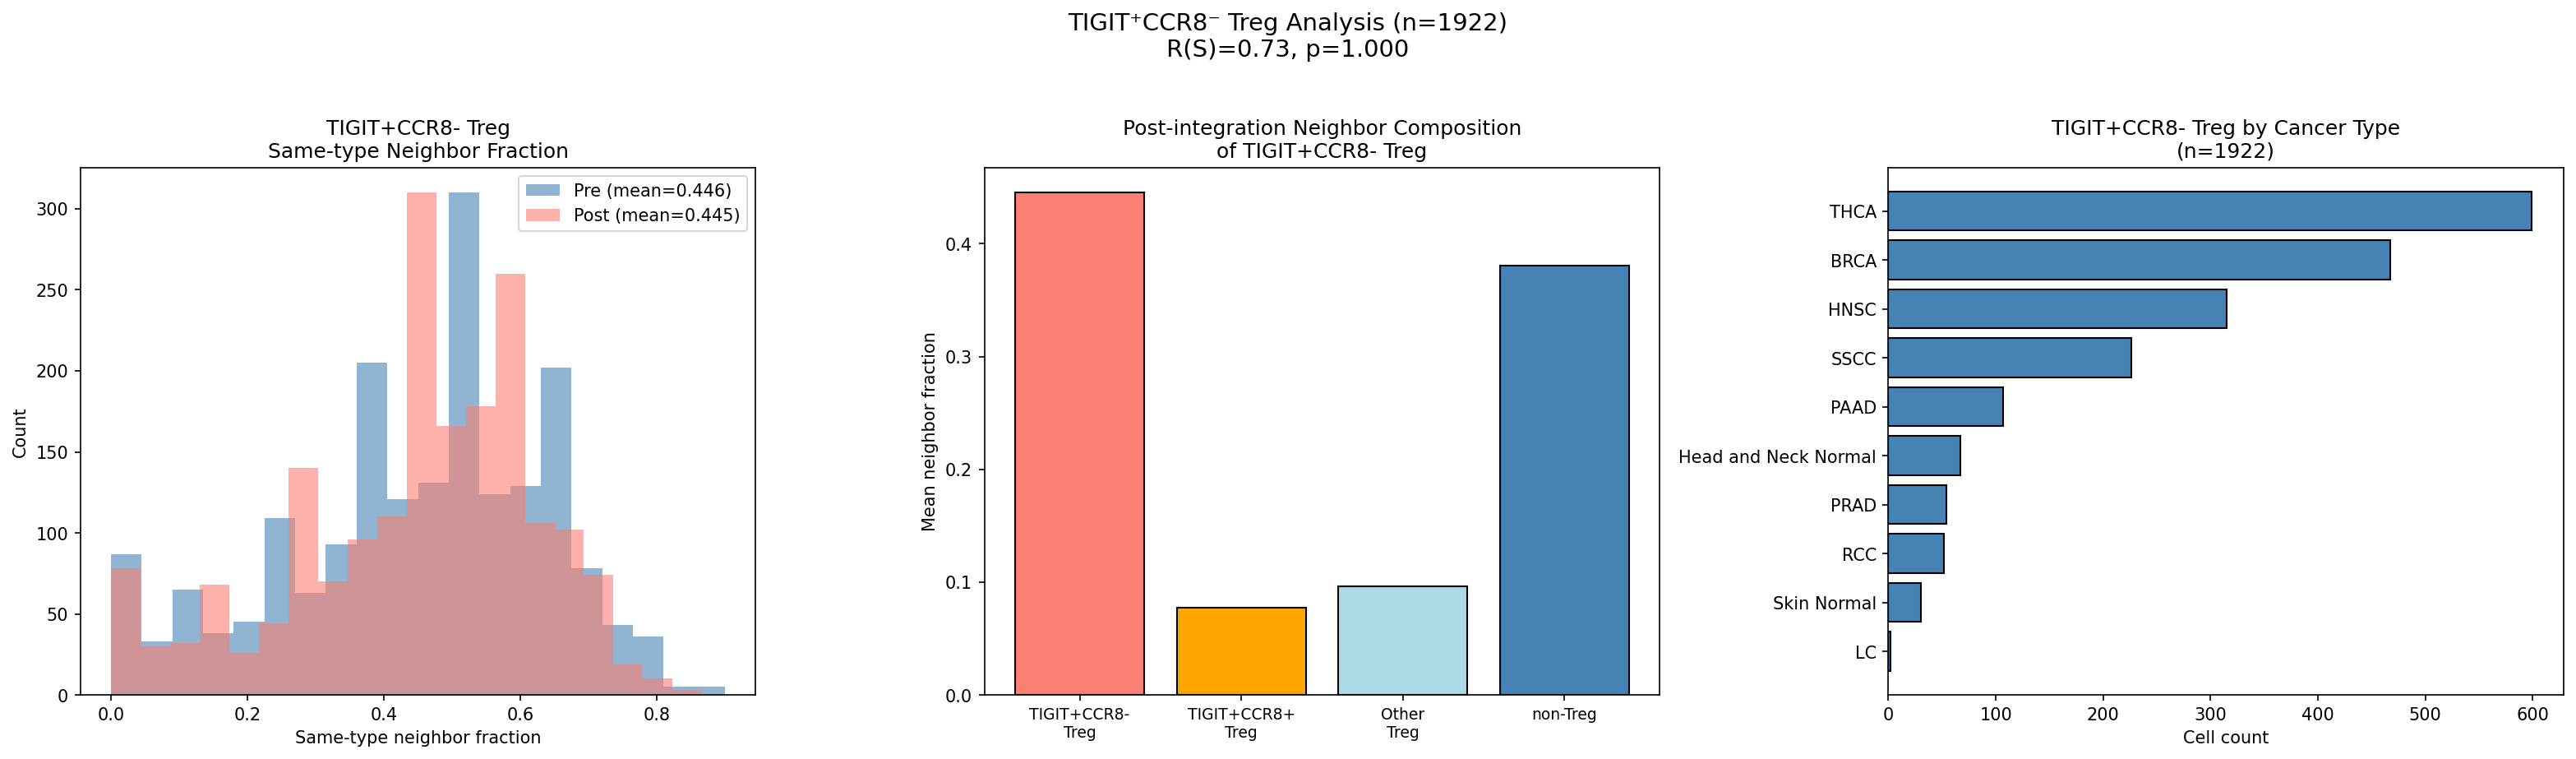
\includegraphics[width=0.8\textwidth]{fig16_tigit_ccr8_treg}
\caption{\textbf{Extended Data Fig.~4:} TIGIT$^+$CCR8$^-$ Treg distribution across T cell subclusters.}
\end{figure}

\begin{figure}[!ht]
\centering
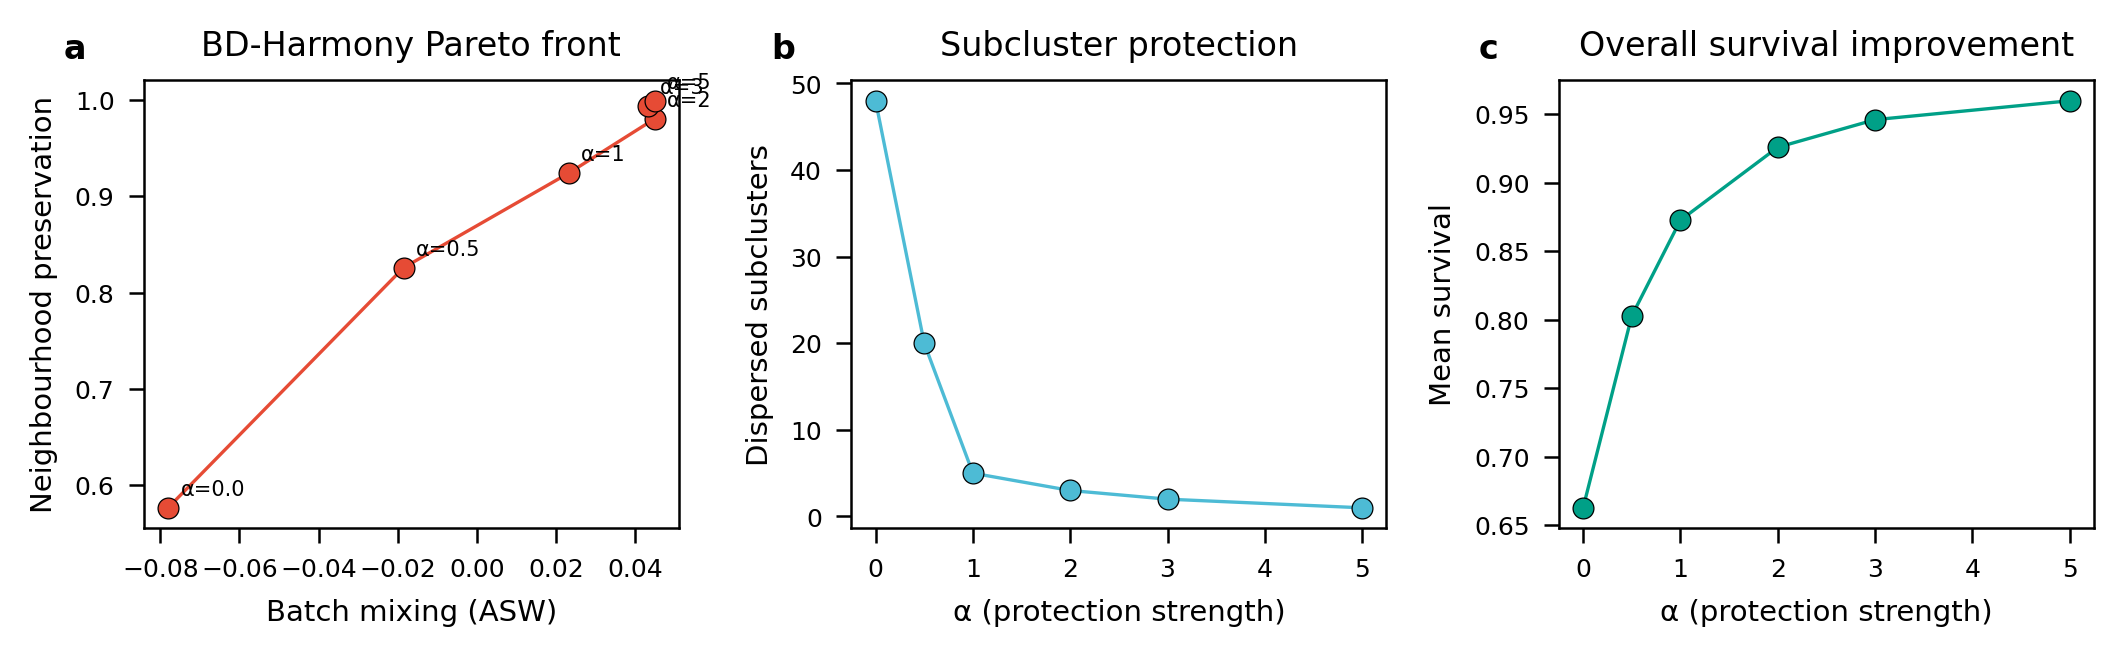
\includegraphics[width=0.8\textwidth]{Fig5_BD_pareto}
\caption{\textbf{Extended Data Fig.~5:} BD-Harmony Pareto frontier (NP vs batch ASW for varying BD weights).}
\end{figure}

\begin{figure}[!ht]
\centering
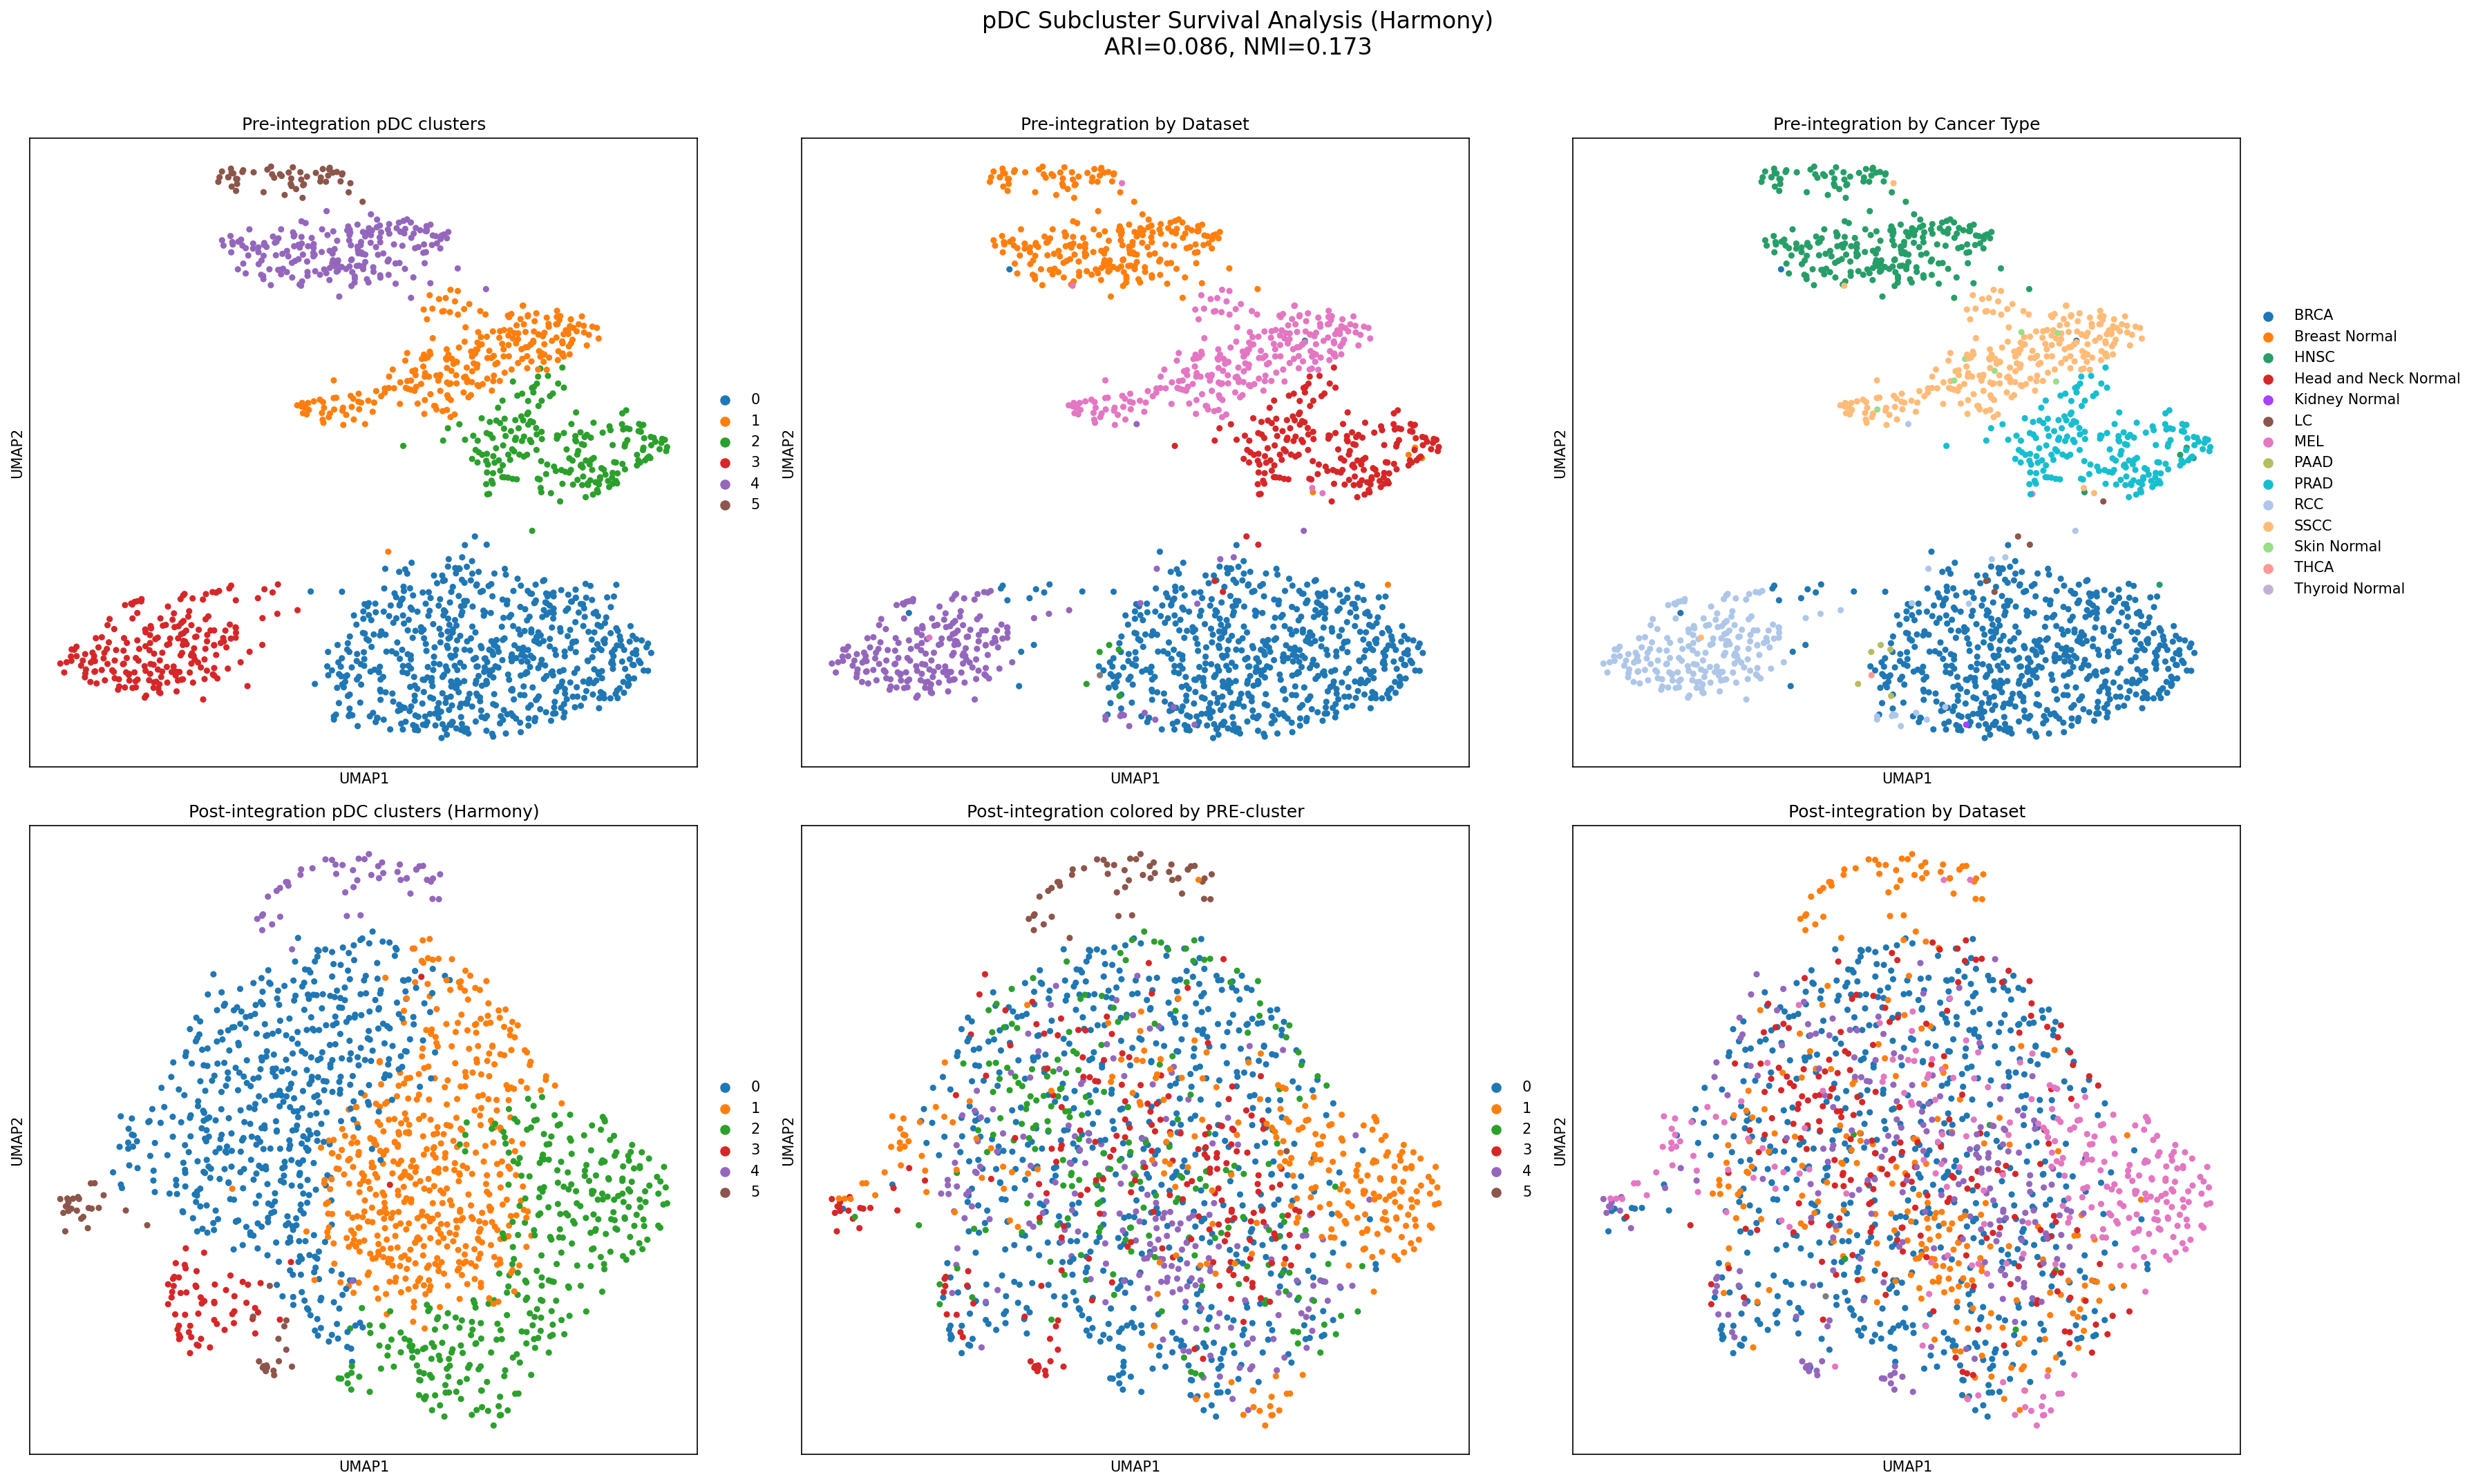
\includegraphics[width=0.8\textwidth]{fig13_pdc_subcluster_survival}
\caption{\textbf{Extended Data Fig.~6:} pDC subcluster survival analysis (6 pre-integration subclusters, ARI=0.09).}
\end{figure}

\begin{figure}[!ht]
\centering
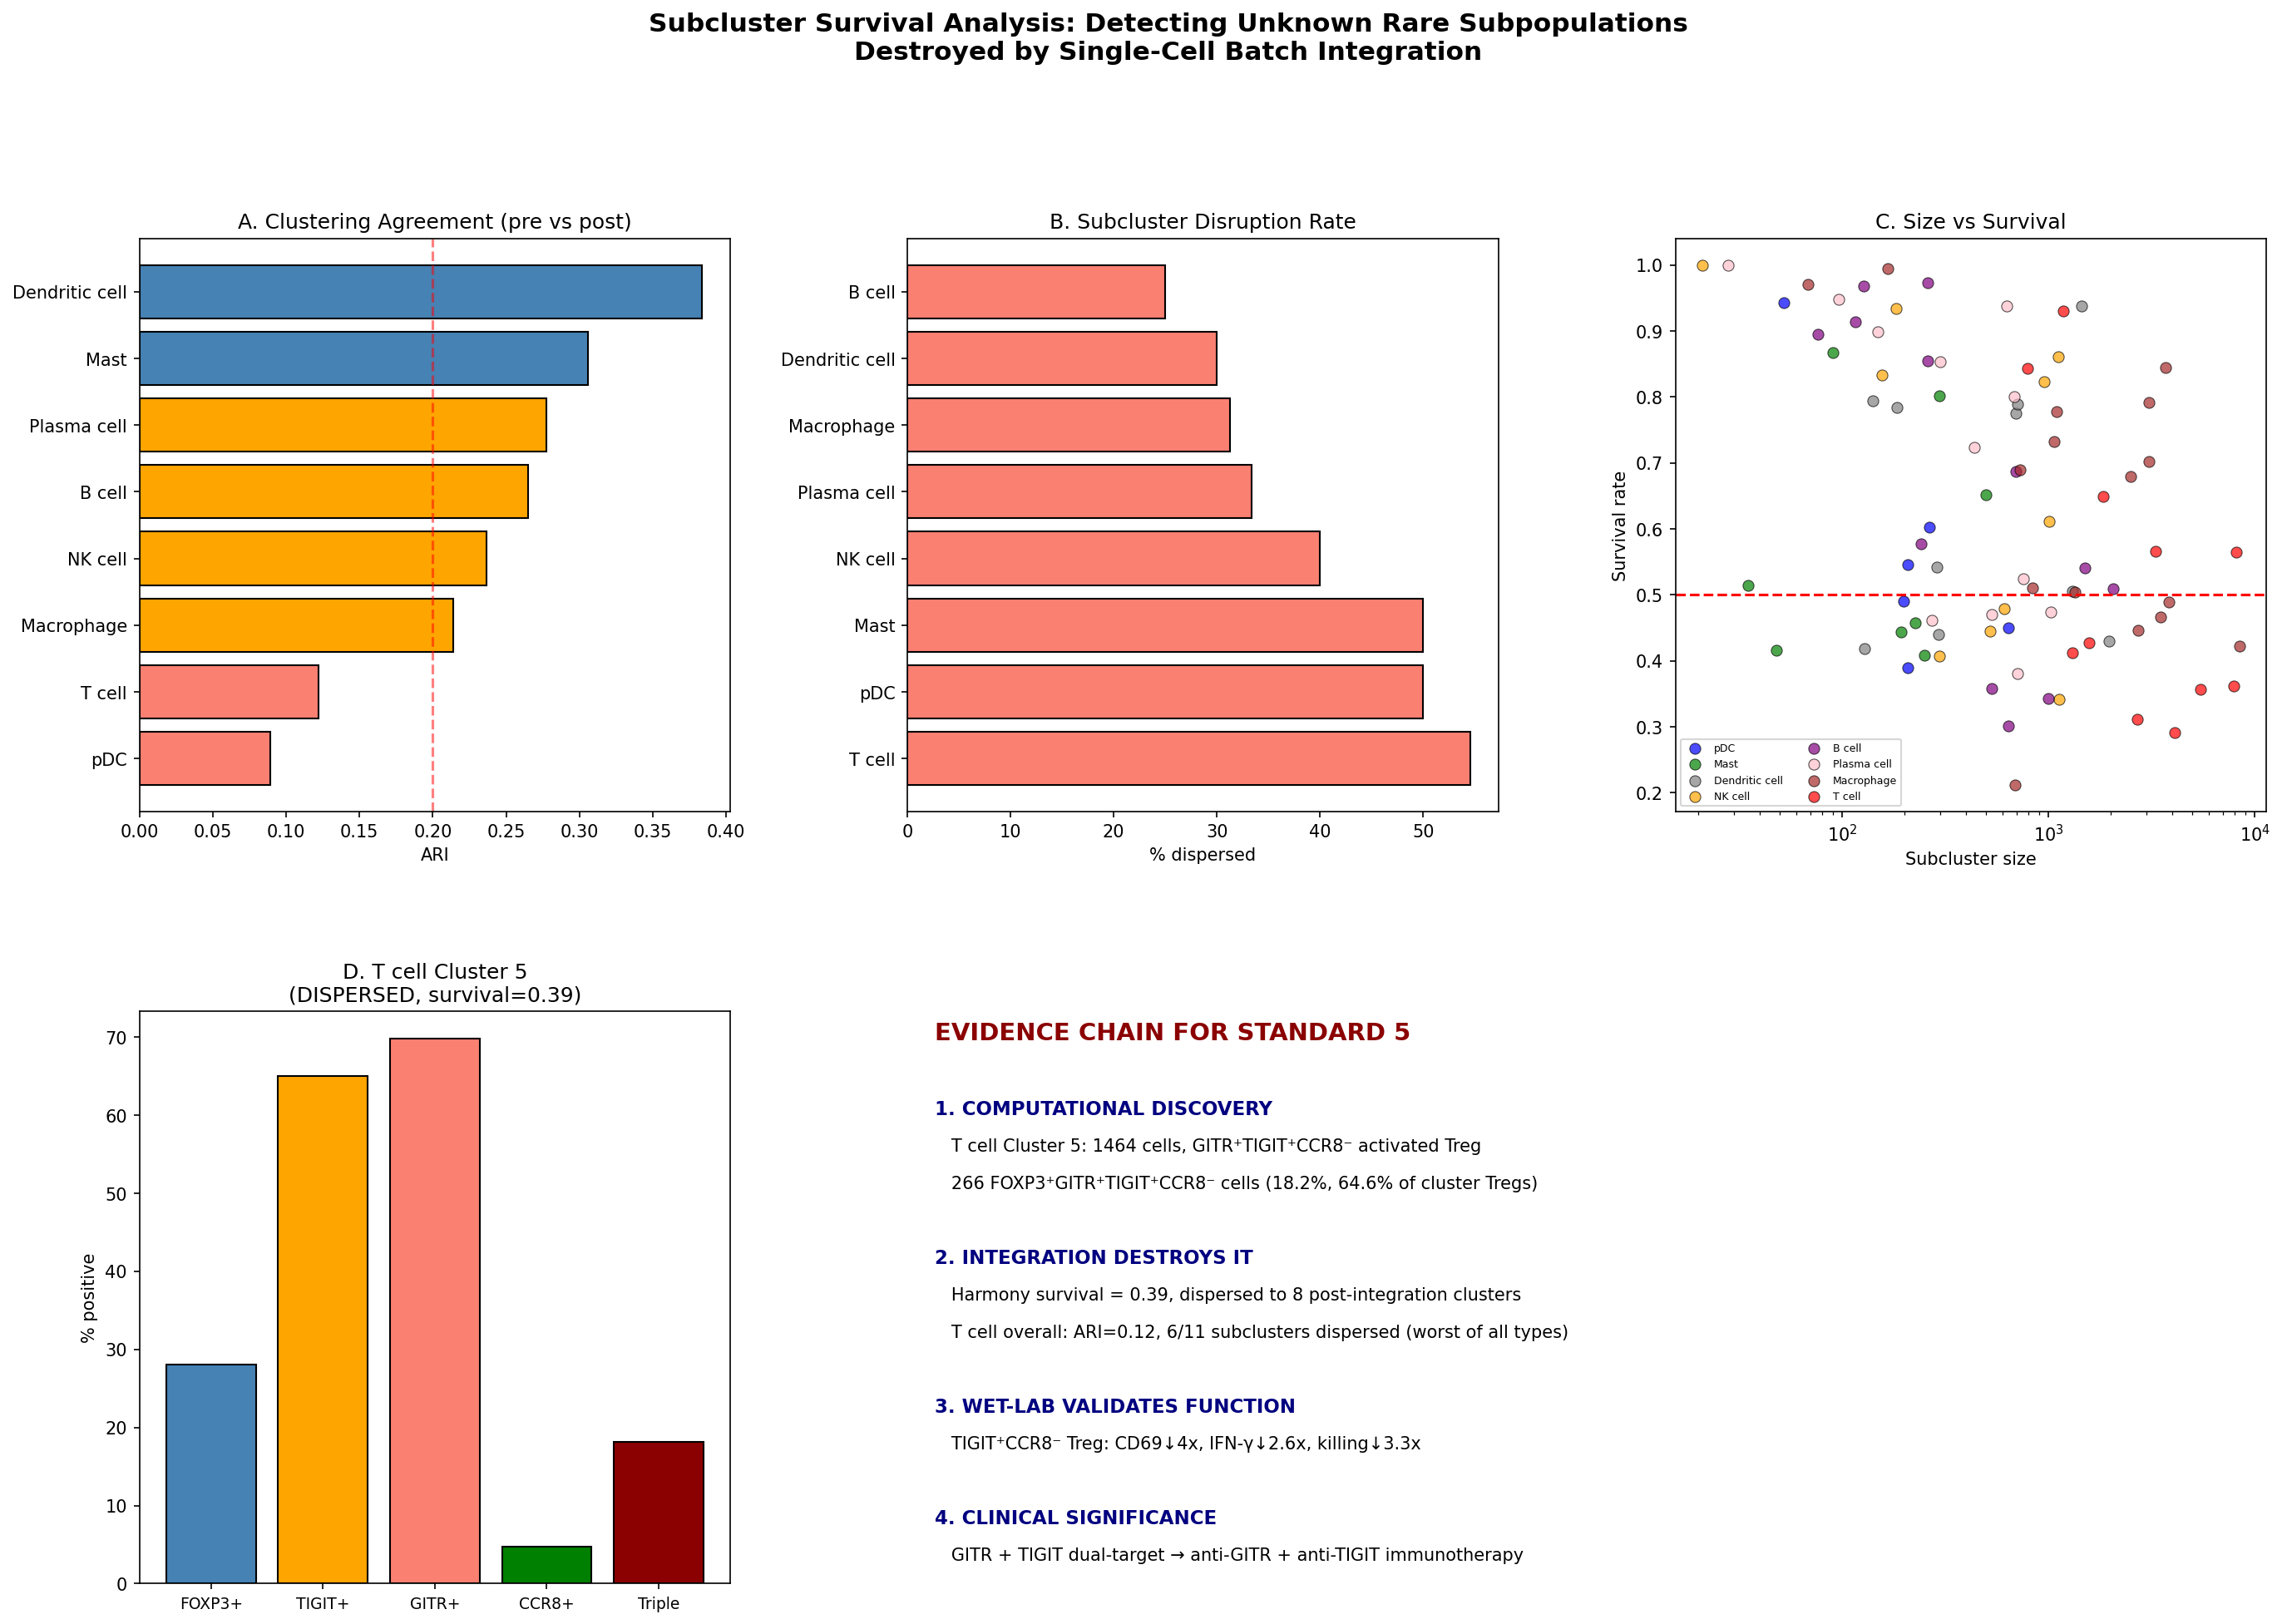
\includegraphics[width=0.8\textwidth]{fig20_framework_validation_summary}
\caption{\textbf{Extended Data Fig.~7:} Framework validation summary and standard 5 evidence chain.}
\end{figure}

\begin{figure}[!ht]
\centering
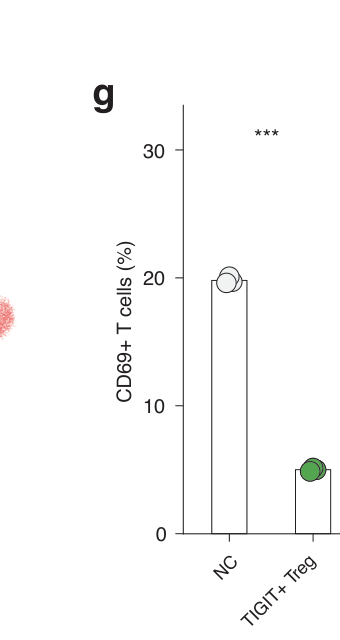
\includegraphics[width=0.32\textwidth]{fig5g_CD69}
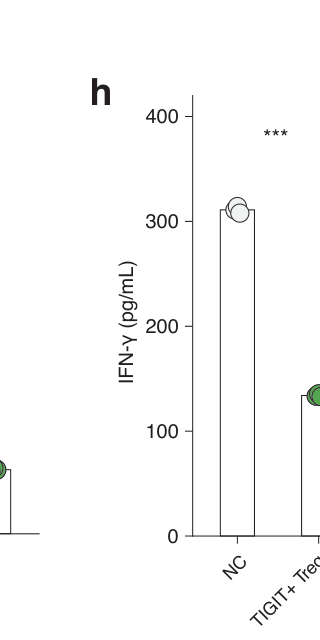
\includegraphics[width=0.32\textwidth]{fig5h_IFNg}
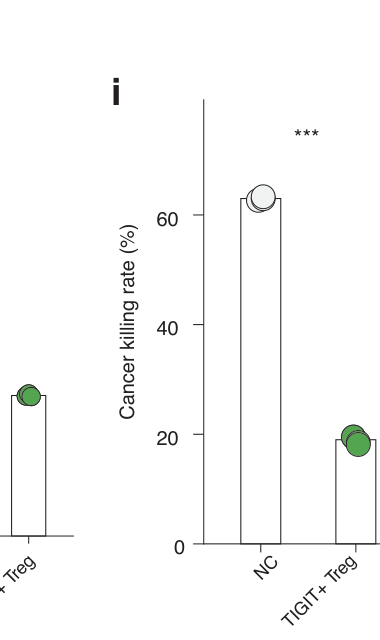
\includegraphics[width=0.32\textwidth]{fig5i_killing}
\caption{\textbf{Extended Data Fig.~8:} Original wet-lab data: CD69 flow cytometry (left), IFN-$\gamma$ ELISA (center), LDH killing assay (right).}
\end{figure}

\paragraph{Extended Data Fig.~1 $|$ Signal retention per pipeline step.}
Measured retention of rare-type marker gene expression signal across 5 pipeline steps (raw $\to$ QC $\to$ HVG $\to$ PCA $\to$ Harmony) for 4 cell types. pDC drops to 40\% at HVG step; Mast retains 100\% through HVG but drops to 63.8\% at Harmony.

\paragraph{Extended Data Fig.~2 $|$ BD distribution across cell types.}
Histogram of per-cell BD scores for 105k immune subset, colored by cell type. Mean BD = 0.179; Mast highest (0.244), Plasma lowest (0.155).

\paragraph{Extended Data Fig.~3 $|$ KAN vs.\ linear BD weighting.}
Comparison of integration weight strategies: linear BD (NP = 0.890) vs.\ polynomial (NP = 0.872). Linear weighting is sufficient; nonlinear alternatives provide no improvement.

\paragraph{Extended Data Fig.~4 $|$ Full atlas (4.83M) per-celltype NP.}
Bar chart of mean NP by cell type at full atlas scale. Clear separation between immune (0.47--0.53) and non-immune (0.62--0.75) lineages.

\paragraph{Extended Data Fig.~5 $|$ Phase transition power-law fits.}
NP versus batch count with power-law sigmoid fits ($R^2 > 0.98$) for 8 immune cell types, with annotated $B_{50}$ half-life values.

\end{document}
